\section{React Native CLI}
\textbf{Wichtig}: In der Installationsanleitung auf der Webseite von React Native kann man sein
aktuelles Betriebssystem und Zielplattform auswählen. Apple erlaubt nicht die Entwicklung von Apps
auf anderen Betriebssystemen als MacOS selbst, d.h. die Entwicklung der iOS-App ist auf Windows 11,
meinem Betriebssystem, nicht möglich. Ich hatte während der Entwicklung nie Zugriff auf einen PC mit
MacOS, daher wurde die gesamte App ausschließlich für Android entwickelt. Doch sollten wir jemals
diese App wirklich veröffentlichen wollen, so wird das Umschreiben keinen großen Aufwand darstellen,
da wir immer darauf geachtet haben, nur Bibliotheken zu verwenden, die auch für iOS kompatibel sind.

\subsection{Abhängigkeiten und Erstellung des Projekts}
Für die Verwendung der React-Native-CLI werden einige andere Softwarepakete benötigt, darunter --
natürlich -- \nameref{nodejs}, mindestens Version 12. Außerdem wird benötigt:

\begin{itemize}
  \item Java SE Development Kit (mind. Version 11)
  \item Android Studio
  \begin{itemize}
    \item Android SDK 11 (R)
    \item Android SDK Platform: API Level 30
    \item Android Virtual Device: Google Pixel 2 mit Android 11
  \end{itemize}
\end{itemize}

Sobald alle Abhängigkeiten installiert wurden, führt man folgenden Befehl aus, um ein neues React
Native Projekt zu erstellen:

\begin{lstlisting}
C:\example> npx react-native init reactNativeInit
\end{lstlisting}

NPX ist ein Befehl, der seit Version 5.2.0 in NPM enthalten ist. Er ist speziell bei CLIs hilfreich,
denn anstatt das Paket react-native auf dem PC zu installieren und dann aufzurufen, wird mit dem
Befehl automatisch die neueste Version der CLI von einem Server abgefragt und ausgeführt. So kann
man sicherstellen, dass niemals eine veraltete Version der CLI verwendet wird.

\subsubsection{Metro}
\label{metrobundler}
Beim Start der App wird als erstes der Metro Bundler initialisiert. Er besteht aus einem Server,
welcher den geschriebenen Code mittels Babel kompiliert und anschließend an die App schickt. Dadurch
verhindert man, jedes mal die App neu auf das Gerät installieren zu müssen, um eine kleine Änderung
im Text sehen zu können. Beim Einbinden von neuen JavaScript-Bibliotheken muss allerdings der
Bundler neu gestartet werden, um diese verwenden zu können.

Um den Server zu starten gibt man folgenden Befehl ein:

\begin{lstlisting}
C:\example\reactNativeInit> npm start
\end{lstlisting}

Dies ist die Kurzschreibweise für den Befehl npm run start. Start ist nämlich ein Skript in der
Datei package.json.

\begin{figure}[H]
  \begin{center}
    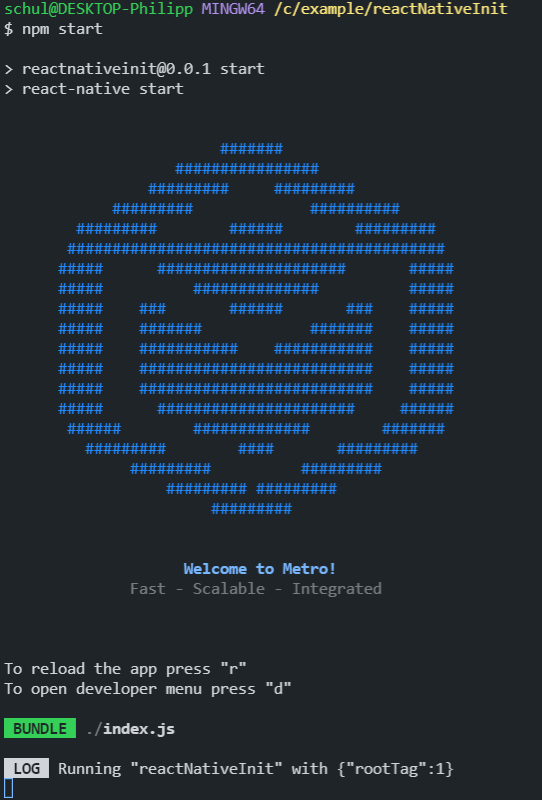
\includegraphics[width=0.5\textwidth]{Theorie/ReactNative/MetroBundler.png}
    \caption{Der Metro-Server in Aktion}
  \end{center}
\end{figure}

Als nächstes öffnet man den Ordner root/android in Android Studio. Man hat nun zwei Möglichkeiten,
die App auszuführen:

\begin{enumerate}
  \item Mit einem virtuellen Android Gerät (Android Virtual Device AVD):\\
Dazu öffnet man in Android Studio den AVD-Manager und erstellt einen neuen Emulator mit einer
Android Version von 11. Danach startet man den Emulator und führt folgenden Befehl aus:

\begin{lstlisting}
C:\example\reactNativeInit> npm run android
\end{lstlisting}

Die App wird auf dem Emulator installiert und ausgeführt.

\begin{figure}[H]
  \begin{center}
    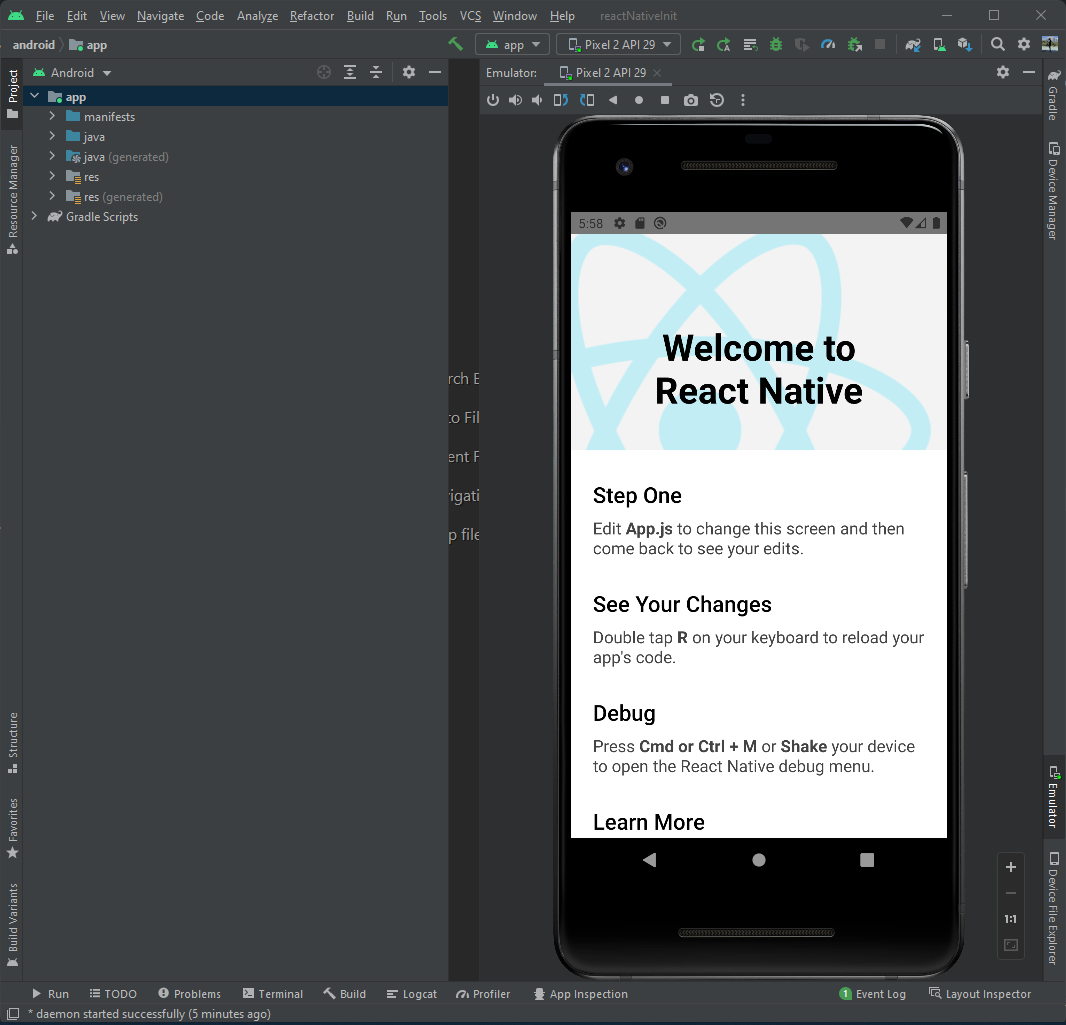
\includegraphics[width=0.8\textwidth]{Theorie/ReactNative/AndroidStudio.png}
    \caption{Die Beispiel-App in Android Studio}
  \end{center}
\end{figure}

  \item Mit einem physischen Android-Gerät:\\
Als erstes aktiviert man auf dem Gerät in den Einstellungen USB-Debugging und schließt es mittels
USB an den PC an. Wenn alle Treiber installiert sind, müsste es dann direkt in Android Studio
erkannt werden, um die App zu installieren.

Jetzt muss noch ein Tunnel über die USB-Verbindung erzeugt werden, damit das Gerät darüber mit dem
lokalen Metro-Server kommunizieren kann. Man listet alle Geräte auf und erzeugt dann mit der
Device-Identifikation einen Tunnel.

\begin{lstlisting}
C:\example\reactNativeInit> adb devices
List of devices attached
34299o5j85o496g3        device
emulator-8125           device

C:\example\reactNativeInit> adb -s 34299o5j85o496g3 reverse tcp:8081 tcp:8081
8081
\end{lstlisting}

\end{enumerate}